\section{Aktueller Stand der Technik}
\label{sec:chapterexample}
Eine \gls{turklingelanlage} welche Audios und Videos überträgt, ist keine neue Erfindung. Auf dem Markt existieren bereits verschiedene Lösungen und das schon seit mehreren Jahren. Diese sind aber meistens analoge Systeme und verfügen über die Vorteile der Digitalisierung nicht. Die Steuerung über eine Mobileapplikation ist aus diesem Grund bei solchen Lösungen ausgeschlossen.

\begin{figure}[htb!]
	\begin{center}
		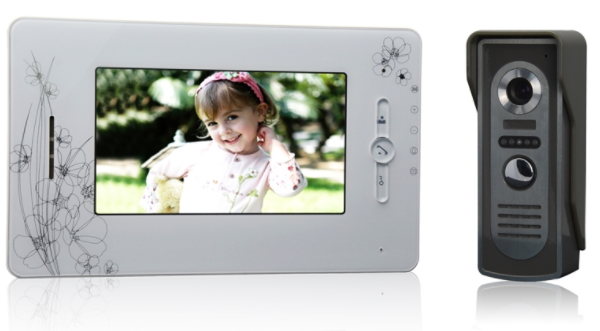
\includegraphics[width=0.66\textwidth]{analog_intercom}
		\caption[Analoge Türsprechanlage mit In-House Display]{Analoge Türsprechanlage mit In-House Display}
		\label{fig:analoge_intercom}
	\end{center}
\end{figure}
In den letzten Jahren sind die ersten, digitalen Lösungen mit \gls{ip} Videoübertragung auf dem Markt gekommen. Die Digitalisierung in diesem Bereich ist den gigantischen Schritten im Bereich der Miniaturisierung und den immer schnelleren Internetzugängen (x\gls{dsl}, \gls{lte}, usw) zu verdanken.

\subsection{Die Herausforderungen der Digitalisierung}
Die Digitalisierung bringt, besonders bei den Video- und Audioübertragungen, nicht nur Vorteile mit sich.  Während eine analoge Videoübertragung ziemlich mühelos erfolgt, muss im Falle einer digitalen Lösung das Video zuerst kodiert und anschliessend wieder dekodiert werden.
\\
Die heutigen Kodierungsalgorithmen ermöglichen eine ziemlich schnelle Dekodierung. Mittlerweile hat jeder Smartphone genug Leistung um ein Full-\gls{dsl} Videostreaming von Youtube oder Netflix in Real Time zu dekodieren. Auf der anderen Seite ist die Kodierung ein sehr rechenintensiver Prozess und benötigt sehr viel Leistung.
\\
Jeder der schon mal mit Video-Editing zu tun hatte, weiss wie viel Zeit das Exportieren eines Videos dauern kann.
\\
Die grösste Herausforderung für die Real Time digitale Video-, Audiokommunikation besteht also darin, die Kodierung und Dekodierung des Audios und Videosignals in vernünftiger Zeit durchzuführen.

\subsection{Marktsituation}
\label{sec:chapterexample}
Das Hauptziel diese Bachelorarbeit ist die Entwicklung einer kostengünstigen Lösung für eine digitale, flexible und skalierbare \gls{turklingelanlage}. Tatsächlich ist es so, dass die bestehende Lösungen sehr teuer sind. Viele Produkte basieren auf Lösungen von Drittanbietern, \gls{sip} Gateways oder andere Elemente die Zusatzkosten verursachen. Das möchten wir alles vermeiden.

\begin{figure}[htb!]
	\begin{center}
		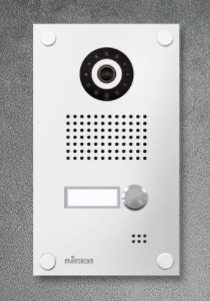
\includegraphics[width=0.33\textwidth]{myintercom}
		\caption[Telecom Behnkle MyIntercom]{Telecom Behnkle MyIntercom}
		\label{fig:myintercom}
	\end{center}
\end{figure}

Eines der günstigsten Produkte das wir finden konnten ist das \textit{"MyIntercom"} von Telecom Behnkle (\seeref{fig:myintercom}). Diese \gls{turklingelanlage} ist ziemlich flexibel und bietet die Möglichkeit, mehrere Türen anzuschliessen. Der Preis liegt, beim Basic-Modell, bei ungefähr 1’600.- CHF pro Türe.
\\
\\
Dank der Aufschwung von Open Source Hardware wie das Raspberry PI und Real Time Communication Protokolle wie \gls{webrtc} muss es möglich sein, kostengünstigere Lösungen zu erarbeiten. In den folgenden Kapiteln geht es nun um die effektive Realisierung eines Prototyps, welcher die oben genannte Problemen adressiert.
\newpage